\chapter{Appendix}
\label{sec:Appendix}
\section{Iperf3 Testergebnisse}
\makeatletter
\setlength{\@fptop}{0pt}
\makeatother
\begin{table}[hp]
\centering
\large
\begin{tabular}{c||c c c c c}
Paketgröße & Baseline & AES-GCM & AEGIS128L & ChaCha20-Poly1305 & MORUS640  \\
\hline  
in bytes & \multicolumn{4}{c}{in mbytes/s} \\
\hline 
128 & 560.89 & 405.67 & 279.42 & 411.31 & 220.18  \\ 
256 & 856.55 & 773.62 & 620.32 & 773.34 & 498.61  \\ 
512 & 1038.22 & 981.99 & 968.6 & 981.89 & 854.6 \\ 
1024 & 1138.45 & 1107.16 & 1099.26 & 1107.10 & 1099.25  \\ 
1400 & 1136.97 & 1143.71 & 1137.6 & 1143.61 & 1136.93 \\
1514 & 1145.89 & 1152.72 & 1146.48 & 1152.51 & 1145.89 \\  
\end{tabular}
\centering \caption[Datenübertragungsrate mit Verschlüsselung]{ Die Bandbreite in mbyte/s mit Verschlüsselung.}
\label{tab:bytes-e}
\end{table}

\begin{table}[hp]
\centering
\large
\begin{tabular}{c||c c c c c}
Paketgröße & Baseline & AES-GCM & AEGIS128L & ChaCha20-Poly1305 & MORUS640  \\
\hline  
in bytes & \multicolumn{4}{c}{in mbytes/s} \\
\hline
128 & 560.89 & 408.04 & 286.94 & 406.62 & 233.43  \\ 
256 & 856.55 & 774.06 & 651.54 & 773.45 & 535.74  \\ 
512 & 1038.22 & 982.04 & 1107.23 & 981.93 & 938.27 \\ 
1024 & 1138.45 & 1107.12 & 1143.69 & 1107.16 & 1107.38  \\ 
1400 & 1136.97 & 1143.67 & 1137.6 & 1143.65 & 1143.36 \\
1514 & 1145.89 & 1152.69 & 1152.1 & 1152.52 & 1152.21 \\  
\end{tabular} 
\centering \caption[Datenübertragungsrate ohne Verschlüsselung]{ Die Bandbreite in mbyte/s ohne Verschlüsselung.}
\label{tab:bytes-we}



\end{table}
\begin{table}[hp]
\centering
\large
\begin{tabular}{c||c c c c c}
Paketgröße & Baseline & AES-GCM & AEGIS128L & ChaCha20-Poly1305 & MORUS640  \\
\hline  
in bytes & \multicolumn{4}{c}{in Prozent} \\
\hline
128 & 0.91 & 1.13 & 40.39 & 96.63 & 93.13  \\ 
256 & 1.21 & 1.34 & 3.04 & 2.32 & 98.04  \\ 
512 & 1.41 & 1.4 & 2.19 & 1.58 & 99.41 \\ 
1024 & 1.60 & 1.39 & 1.81 & 1.51 & 3.88  \\ 
1400 & 1.55 & 1.11 & 1.22 & 1.16 & 1.93 \\
1514 & 1.5 & 1.11 & 1.22 & 1.15 & 1.84 \\  
\end{tabular} 
\caption[CPU Auslastung mit Verschlüsselung]{ Die CPU Auslastung in Prozent mit Verschlüsselung.}
\label{tab:CPU-e}
\end{table}
\begin{table}[htp]
\centering
\large
\begin{tabular}{c||c c c c c}
Paketgröße & Baseline & AES-GCM & AEGIS128L & ChaCha20-Poly1305 & MORUS640  \\
\hline
in bytes & \multicolumn{4}{c}{in Prozent} \\
\hline  
128 & 0.91 & 1.08 & 33.15 & 92.39 & 89.04  \\ 
256 & 1.21 & 1.35 & 1.96 & 2.32 & 89.87  \\ 
512 & 1.41 & 1.4 & 1.95 & 1.57 & 99.39 \\ 
1024 & 1.60 & 1.41 & 1.72 & 1.5 & 3.3  \\ 
1400 & 1.55 & 1.12 & 1.21 & 1.14 & 1.54 \\
1514 & 1.5 & 1.12 & 1.2 & 1.15 & 1.51 \\  
\end{tabular} 

\caption[CPU Auslastung ohne Verschlüsselung]{ Die CPU Auslastung in Prozent ohne Verschlüsselung.}
\label{tab:CPU-we}
\end{table}
\clearpage
\section{ping Testergebnisse}
\begin{table}[h]
\large
\begin{tabular}{c||c c c c c}
Paketgröße & Baseline & AES-GCM & AEGIS128L & ChaCha20-Poly1305 & MORUS640  \\
\hline  
in bytes & \multicolumn{4}{c}{in ms} \\
\hline 
128 & 0.136 & 0.143 & 0.147 & 0.149 & 0.152  \\ 
256 & 0.14 & 0.144 & 0.148 & 0.15 & 0.154  \\ 
512 & 0.142 & 0.144 & 0.161 & 0.152 & 0.16 \\ 
1024 & 0.146 & 0.146 & 0.174 & 0.153 & 0.17  \\ 
1514 & 0.15 & 0.147 & 0.181 & 0.154 & 0.177 \\
\end{tabular}
\caption[Paketumlaufzeit mit Verschlüsselung]{Die durchschnittlichen Paketumlaufzeiten mit Verschlüsselung in ms.}
\label{tab:Lat-e}
\end{table}

\begin{table}[h]
\large
\begin{tabular}{c||c c c c c}
Paketgröße & Baseline & AES-GCM & AEGIS128L & ChaCha20-Poly1305 & MORUS640  \\
\hline  
in bytes & \multicolumn{4}{c}{in ms} \\
\hline 
128 & 0.136 & 0.141 & 0.148 & 0.148 & 0.15  \\ 
256 & 0.14 & 0.145 & 0.147 & 0.148 & 0.153  \\ 
512 & 0.142 & 0.149 & 0.15 & 0.149 & 0.157 \\ 
1024 & 0.146 & 0.155 & 0.155 & 0.15 & 0.166  \\ 
1514 & 0.15 & 0.161 & 0.159 & 0.151 & 0.17 \\
\end{tabular}
\caption[Paketumlaufzeit ohne Verschlüsselung]{Die durchschnittlichen Paketumlaufzeiten ohne Verschlüsselung in ms.}
\label{tab:Lat-we}
\end{table}

\begin{figure}[!p]
\centering
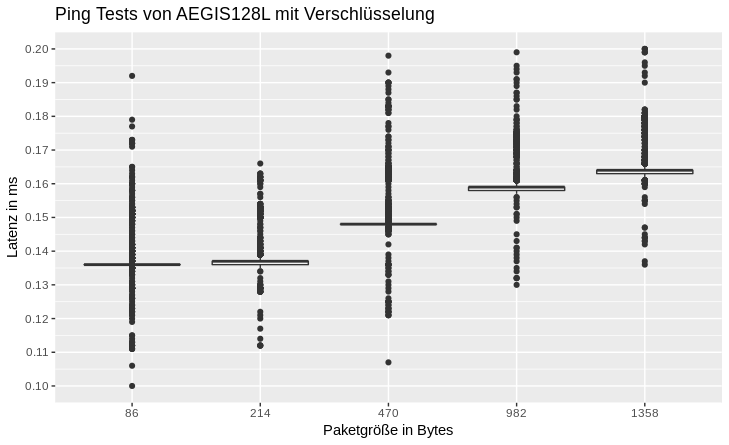
\includegraphics[width=0.95\textwidth]{images/aegiseping.png}
\caption[Ping Diagramm mit AEGIS128L mit Verschlüsselung]{Das Boxplot Diagramm zeigt die Ping Tests mit dem Verschlüsselungsalgorithmus AEGIS128L. Es wurden 50.000 Tests durchgeführt. Es wurde mit Verschlüsselung getestet. }
\label{img:AEGISping}
\end{figure}
\begin{figure}[!p]
\centering
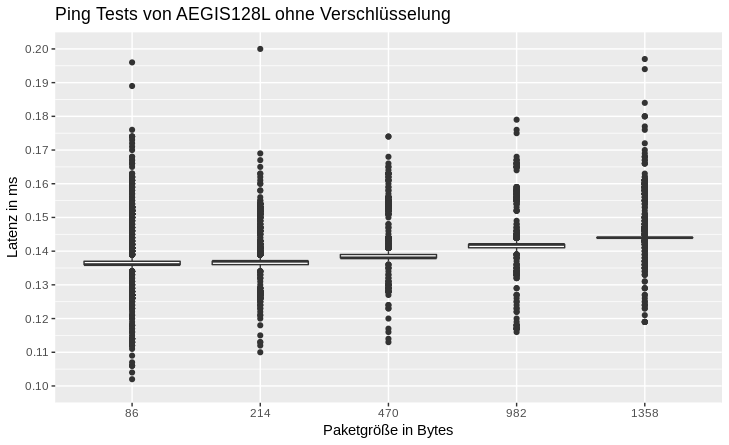
\includegraphics[width=0.95\textwidth]{images/aegisweping.png}
\caption[Ping Diagramm mit AEGIS128L ohne Verschlüsselung]{Das Boxplot Diagramm zeigt die Ping Tests mit dem Verschlüsselungsalgorithmus AEGIS128L. Es wurden 50.000 Tests durchgeführt. Es wurde ohne Verschlüsselung getestet.  }
\label{img:CPU-WE2}
\end{figure}
\begin{figure}[!p]
\centering
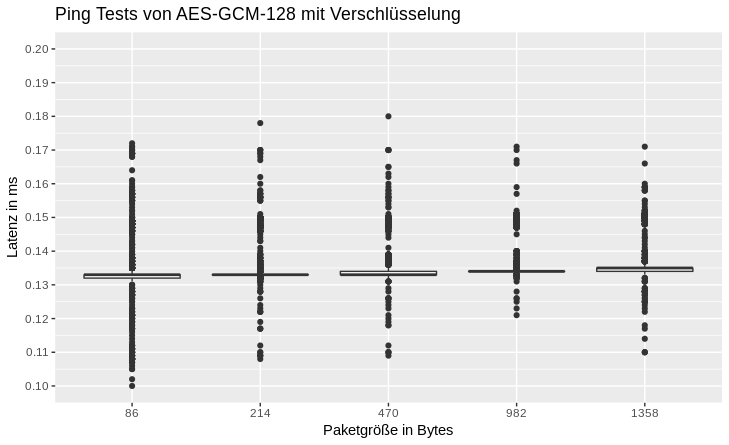
\includegraphics[width=0.95\textwidth]{images/aesEping.png}
\caption[Ping Diagramm mit AES-GCM mit Verschlüsselung]{Das Boxplot Diagramm zeigt die Ping Tests mit dem Verschlüsselungsalgorithmus AES-GCM. Es wurden 50.000 Tests durchgeführt. Es wurde mit Verschlüsselung getestet.  }
\label{img:CPU-WE3}
\end{figure}
\begin{figure}[!p]
\centering
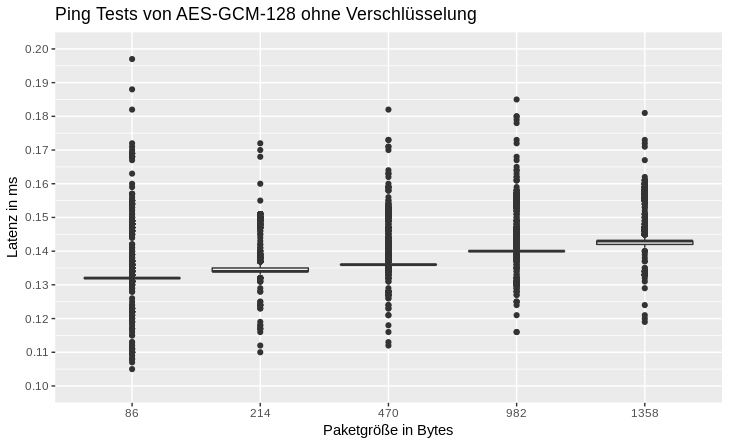
\includegraphics[width=0.95\textwidth]{images/aesWEping.png}
\caption[Ping Diagramm mit AES-GCM ohne Verschlüsselung]{Das Boxplot Diagramm zeigt die Ping Tests mit dem Verschlüsselungsalgorithmus AES-GCM. Es wurden 50.000 Tests durchgeführt. Es wurde ohne Verschlüsselung getestet.  }
\label{img:CPU-WE3}
\end{figure}
\begin{figure}[!p]
\centering
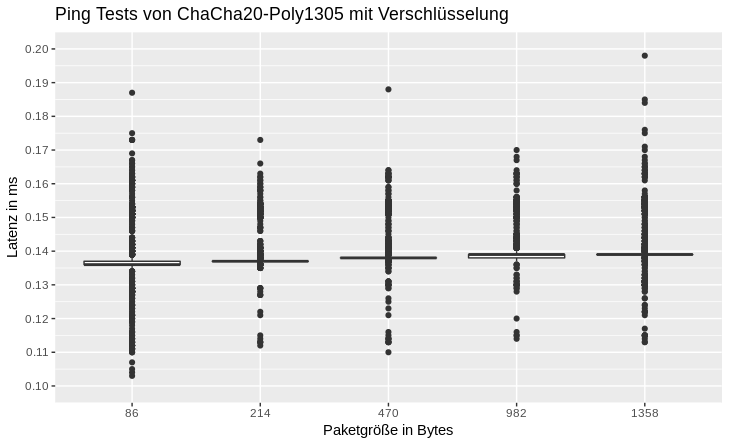
\includegraphics[width=0.95\textwidth]{images/chachaEping.png}
\caption[Ping Diagramm mit ChaCha20-Poly1305 mit Verschlüsselung]{Das Boxplot Diagramm zeigt die Ping Tests mit dem Verschlüsselungsalgorithmus ChaCha20-Poly1305. Es wurden 50.000 Tests durchgeführt. Es wurde mit Verschlüsselung getestet. }
\label{img:CPU-WE4}
\end{figure}
\begin{figure}[!p]
\centering
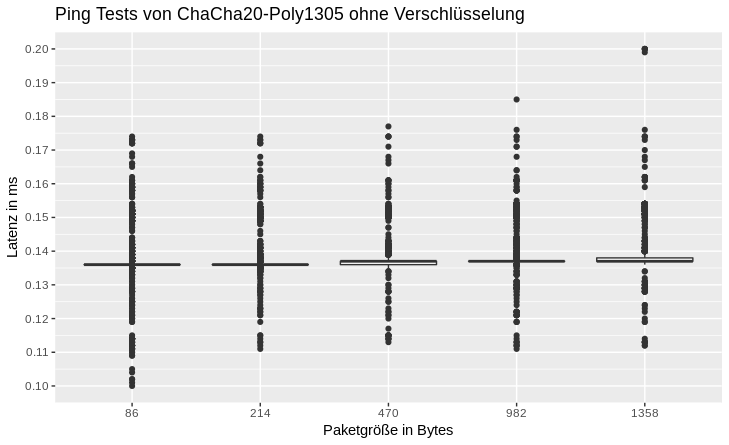
\includegraphics[width=0.95\textwidth]{images/chachaweping.png}
\caption[Ping Diagramm mit ChaCha20-Poly1305 ohne Verschlüsselung]{Das Boxplot Diagramm zeigt die Ping Tests mit dem Verschlüsselungsalgorithmus ChaCha20-Poly1305. Es wurden 50.000 Tests durchgeführt. Es wurde ohne Verschlüsselung getestet. }
\label{img:CPU-WE5}
\end{figure}
\begin{figure}[!p]
\centering
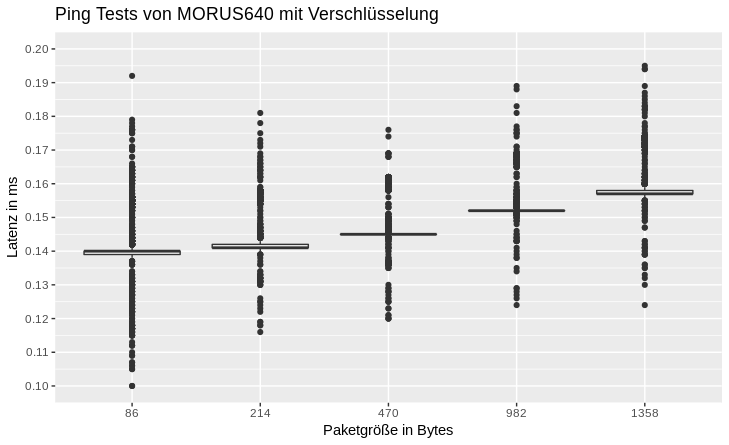
\includegraphics[width=0.95\textwidth]{images/moruseping.png}
\caption[Ping Diagramm mit MORUS640 mit Verschlüsselung]{Das Boxplot Diagramm zeigt die Ping Tests mit dem Verschlüsselungsalgorithmus MORUS640. Es wurden 50.000 Tests durchgeführt. Es wurde mit Verschlüsselung getestet.   }
\label{img:CPU-WE6}
\end{figure}
\begin{figure}[!p]
\centering
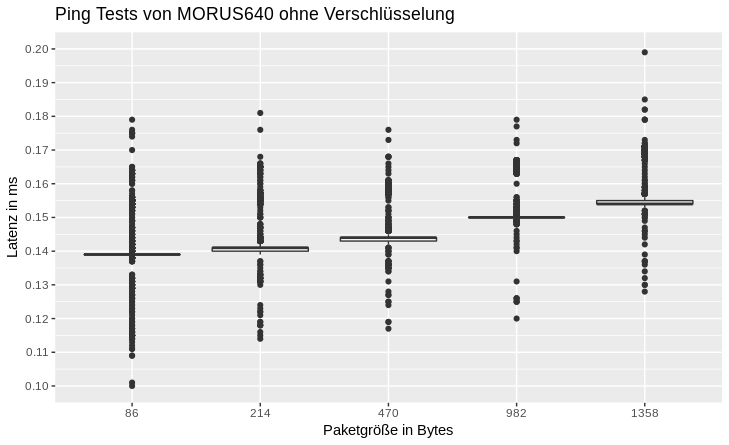
\includegraphics[width=0.95\textwidth]{images/Morusweping.png}
\caption[Ping Diagramm mit MORUS640 ohne Verschlüsselung]{Das Boxplot Diagramm zeigt die Ping Tests mit dem Verschlüsselungsalgorithmus MORUS640. Es wurden 50.000 Tests durchgeführt. Es wurde ohne Verschlüsselung getestet.  }
\label{img:CPU-WE7}
\end{figure}
\begin{figure}[!p]
\centering
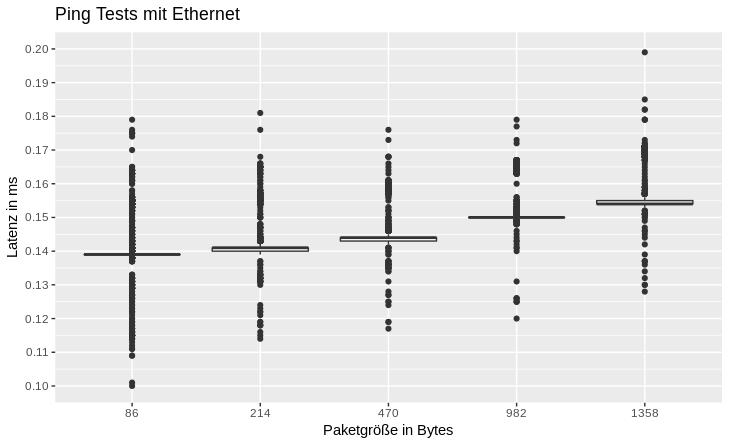
\includegraphics[width=1\textwidth]{images/Ethernetping.png}
\caption[Ping Diagramm mit Ethernet]{Das Boxplot Diagramm zeigt die Ping Tests mit normalen Ethernet Paketen. Es wurden 50.000 Tests durchgeführt. }
\label{img:CPU-WE8}
\end{figure}


\clearpage

%  Schlußfolgerungen, Fragen, Ausblicke

% Dieses Kapitel ist sicherlich das am Schwierigsten zu schreibende. Es
% dient einer gerafften Zusammenfassung dessen, was man gelernt hat. Es
% ist möglicherweise gespickt von Rückwärtsverweisen in den Text, um dem
% faulen aber interessierten Leser (der Regelfall) doch noch einmal die
% Chance zu geben, sich etwas fundierter weiterzubilden. Manche guten
% Arbeiten werfen mehr Probleme auf als sie lösen. Dies darf man ruhig
% zugeben und diskutieren. Man kann gegebenenfalls auch schreiben, was
% man in dieser Sache noch zu tun gedenkt oder den Nachfolgern ein paar
% Tips geben. Aber man sollte nicht um jeden Preis Fragen, die gar nicht
% da sind, mit Gewalt aufbringen und dem Leser suggerieren, wie
% weitsichtig man doch ist. Dieses Kapitel muß kurz sein, damit es
% gelesen wird.


%%% Local Variables:
%%% TeX-master: "diplom"
%%% End:
